\documentclass{article}

\usepackage{corl_2026} % Initial submission (anonymized)
% \usepackage[final]{corl_2026}    % Camera-ready
% \usepackage[preprint]{corl_2026} % arXiv preprint

\usepackage{amsmath,amssymb,amsfonts}
\usepackage{booktabs}
\usepackage{multirow}
\usepackage{graphicx}
\usepackage{xcolor}
\usepackage{microtype}

% -----------------------------------------------------------------------
% Draft helpers — remove before submission
\newcommand{\todo}[1]{\textcolor{red}{\textbf{[TODO: #1]}}}
\newcommand{\placeholder}[1]{\textcolor{gray}{\textit{[#1]}}}
% -----------------------------------------------------------------------

\title{Reward Engineering Playbook:\\
A Systematic Study of Dense Reward Geometry\\
for Robot Manipulation}

\author{Anonymous CoRL 2026 Submission}

\begin{document}
\maketitle

% -----------------------------------------------------------------------
\begin{abstract}
Dense reward design for robot manipulation is a persistent bottleneck: small changes
in reward formulas can produce qualitatively different learning outcomes, yet the field
lacks principled guidance for making these choices. Existing approaches either rely on
trial and error or use black-box tools (e.g., LLM-generated rewards) that improve
iteration speed without explaining \emph{why} particular formulations succeed or fail.
We present a systematic empirical study of dense reward geometry across four independently
controllable dimensions---reaching-shape family, stage gating mechanism, terminal bonus
structure, and normalization---using ManiSkill3's tabletop manipulation suite as a
controlled testbed. By injecting reward variants as environment parameters and holding
algorithms, tasks, and infrastructure fixed, we isolate the causal effect of reward
geometry on learning dynamics. Experiments across four tasks reveal a fundamental
\emph{robustness-ceiling tradeoff}: finite-support rewards resist hard initialisations
but cause mode-switching instability, while infinite-support rewards are stable but
trap policies in hover attractors. Within-episode scale annealing (\texttt{adaptive\_tanh\_episode})
resolves this tradeoff on flat tasks (PickCube: $0.979 \pm 0.029$, PushCube: $0.958$,
LiftPegUpright: $0.854$) but catastrophically fails on hierarchical tasks
(StackCube: $0.021$ vs.\ $0.896$ for finite-support). This complete ranking inversion
motivates \texttt{adaptive\_tanh\_stage}: stage-conditioned annealing that resets
the curriculum clock at each task-stage transition, predicted to unify both regimes.
The outcome is a \emph{reward engineering playbook}---empirically grounded guidance
for selecting dense reward functions by task structure.
\end{abstract}

\keywords{reward shaping, dense rewards, robot manipulation, reinforcement learning,
reward design, empirical study}

% -----------------------------------------------------------------------
\section{Introduction}
\label{sec:intro}

Reinforcement learning for robot manipulation requires dense reward functions to guide
exploration: purely sparse rewards that fire only at success are rarely sufficient for
contact-rich, multi-stage tasks. Yet practitioners designing these dense rewards have
few principled guidelines. The standard approach is to write a distance-based potential
that decreases toward the goal, add binary stage bonuses, and tune scale factors
empirically until training converges. This process is slow, non-transferable, and yields
little understanding of which mathematical properties of the reward function matter.

The question we study is: \emph{given that the task and algorithm are fixed, how does
the geometry of the dense reward function---its shape, curvature, support, smoothness,
and staging---causally affect learning dynamics and final performance?}

This is distinct from several related lines of work. Automated reward generation
methods~\citep{ma2024eureka} improve the speed of reward iteration but treat reward code
as a black box to be searched rather than a structured object to be understood.
Reward shaping theory~\citep{ng1999shaping,devlin2012potential} provides guarantees
about policy invariance under specific transformations but says little about optimization
speed or empirical ranking among non-equivalent reward functions. What is missing is a
controlled, systematic empirical study of reward geometry under on-policy learning in
manipulation.

We address this gap by decomposing dense manipulation rewards into four independently
parameterizable dimensions (\S\ref{sec:taxonomy}), implementing them as environment
kwargs in ManiSkill3 (\S\ref{sec:setup}), and sweeping across combinations while
holding everything else fixed.

\paragraph{Contributions.}
\begin{itemize}
    \item A taxonomy of dense reward geometry along four axes, with concrete
    implementations for 11 ManiSkill3 tabletop tasks
    (Appendix~\ref{app:tasks}).
    \item Multi-seed experiments ($3\times$ seeds, 5--40M steps) on four tasks
    spanning flat, rotation-dominated, and hierarchical manipulation.
    \item Identification of a fundamental \emph{robustness-ceiling tradeoff}
    between finite- and infinite-support reward geometry, and its resolution
    via within-episode scale annealing.
    \item A mechanistic account of why time-based annealing fails on hierarchical
    tasks, and a stage-conditioned fix (\texttt{adaptive\_tanh\_stage}).
    \item A reward engineering playbook: recommendations for reward selection
    as a function of task structure (flat vs.\ hierarchical).
    \item \todo{Sim-to-real validation on SO-101 (stretch goal).}
\end{itemize}

% -----------------------------------------------------------------------
\section{Related Work}
\label{sec:related}

\paragraph{Reward shaping theory.}
\citet{ng1999shaping} established that potential-based shaping does not alter the
optimal policy in the limit, but this result does not address optimization dynamics
under finite-sample on-policy methods. \citet{devlin2012potential} extended the theory
to dynamic potential functions. Our work is empirical and focuses on how shaping
geometry affects convergence speed and stability rather than asymptotic correctness.

\paragraph{Automated reward design.}
EUREKA~\citep{ma2024eureka} uses LLMs to generate reward code and refine it via
evolutionary search, achieving impressive results across locomotion and manipulation
tasks. However, the method treats reward formulas as programs to be searched, not as
geometric objects to be understood. Our work is complementary: we aim to understand
\emph{why} certain reward structures work, which could inform better search spaces for
automated methods.

\paragraph{Empirical studies of RL design choices.}
\citet{andrychowicz2020matters} conducted a large-scale study of on-policy RL design
choices (architecture, normalization, etc.) but did not focus on reward geometry.
To our knowledge, no comparable study exists for manipulation-specific reward function
design.

\paragraph{Simulation infrastructure.}
ManiSkill3~\citep{maniskill3} provides GPU-parallelized simulation, a standardized
API across 18+ tabletop manipulation tasks, and built-in support for PPO baselines,
making it ideal for controlled reward geometry sweeps.

\paragraph{Hierarchical task reward design.}
DrS~\citep{zhuang2024drs} learns reusable dense reward functions for multi-stage tasks
by distilling sparse success signals into per-stage dense rewards. Like our work, it
studies stage-decomposed reward design; unlike ours, it focuses on reward
\emph{magnitude} learned from data, not the \emph{functional form} (curvature, support)
analyzed analytically. Hierarchical Potential-Based Reward Shaping (HPRS)~\citep{demir2024hprs}
extends Ng et al.'s potential-based framework to task specifications, but again studies
magnitude via potential functions rather than geometry.
Self-Adaptive Reward Shaping~\citep{selfadaptive2024} adapts reward weights online
but does not study the geometric properties of the shaping function itself.

\paragraph{Hierarchical reinforcement learning.}
Option-Critic~\citep{bacon2017option} and HIRO~\citep{nachum2018hiro} learn temporal
abstractions (options and sub-goals respectively) to decompose hierarchical tasks.
Our approach is complementary: task stages are \emph{given} by the task's
\texttt{evaluate()} function, so we do not need to learn when to switch stages.
We study how the reward geometry within each known stage affects learning.
HER~\citep{andrychowicz2017her} uses goal-conditioned relabeling to handle sparse
rewards; our work instead investigates how the dense shaping geometry interacts with
stage structure.

\paragraph{Curriculum learning.}
Narvekar et al.~\citep{narvekar2020curriculum} provide a framework for curriculum RL
in which training instances are ordered by difficulty. Our within-episode annealing
(\texttt{adaptive\_tanh\_episode}) is a special case of curriculum learning where the
geometry of the reward function itself changes within an episode. The stage-conditioned
extension (\texttt{adaptive\_tanh\_stage}) conditions the curriculum on task progress
rather than wall-clock time.
From Sparse to Dense~\citep{hao2025toddler} motivates sparse-to-dense reward
transitions from biological learning; our adaptive annealing formalizes this intuition
as a within-episode geometric schedule.

\paragraph{Concurrent work.}
Several 2026 preprints explore related but distinct directions: reward landscape
analysis for model-based planning, adaptive reward weighting, and two-stage curriculum
design. These address different algorithmic levers (planning objectives, weight
scheduling, task ordering) rather than the intrinsic geometry of the dense shaping
function itself.

% -----------------------------------------------------------------------
\section{Reward Geometry Taxonomy}
\label{sec:taxonomy}

We decompose dense manipulation rewards into four independently controllable dimensions.
Each dimension is exposed as an environment kwarg (e.g.,
\texttt{reach\_variant="concave\_truncated"}), enabling factorial sweeps without
modifying the algorithm or task.

\subsection{Dimension 1: Reaching Shape}

The reaching component $r_d : \mathbb{R}_{\geq 0} \to \mathbb{R}$ maps
end-effector-to-object distance $d$ to a scalar reward. We study eight static families
and three adaptive variants that vary in curvature, support, and monotonicity
(Table~\ref{tab:reach}).

\begin{table}[h]
\centering
\small
\caption{Reaching reward shape variants. All satisfy $r_d(0) = 1$.
$\nabla r_d|_{d=0}$ is the gradient at the goal.}
\label{tab:reach}
\begin{tabular}{@{}llll@{}}
\toprule
\textbf{Name} & \textbf{Formula} & \textbf{Curvature} & \textbf{$\nabla r|_{d=0}$} \\
\midrule
\texttt{tanh}              & $1 - \tanh(5d)$               & Convex & $-5$ \\
\texttt{linear}            & $\max(0, 1 - 5d)$             & Linear & $-5$ \\
\texttt{exponential}       & $e^{-5d}$                     & Convex & $-5$ \\
\texttt{quadratic}         & $\frac{1}{1+25d^2}$           & Concave peak & $0$ \\
\texttt{tanh\_sq}          & $1 - \tanh(25d^2)$            & Concave, no cutoff & $0$ \\
\texttt{concave\_truncated}& $\max(0,\, 1 - 25d^2)$        & Concave, $r=0$ for $d>0.2$ & $0$ \\
\texttt{oscillatory}       & $(1-\tanh(5d)) + 0.05\sin(20d)$ & Non-monotone & $-5$ \\
\texttt{sparse\_threshold} & $\mathbf{1}[d < 0.05]$        & Discontinuous & --- \\
\midrule
\texttt{adaptive\_tanh\_episode} & $1 - \tanh(k(t)\cdot d)$, $k(t)=2{+}18\tfrac{t}{T}$ & Convex, time-varying & $-k(t)$ \\
\texttt{adaptive\_tanh\_stage}   & $1 - \tanh(k(t_s)\cdot d)$, $k$ resets per stage & Convex, stage-varying & $-k(t_s)$ \\
\bottomrule
\end{tabular}
\end{table}

\subsection{Dimension 2: Stage Gating}

Many manipulation tasks are hierarchical: the robot must reach, then grasp, then place.
We study how the placement reward $r_p$ is conditioned on the grasping phase variable
$c_t \in \{0,1\}$ (or a continuous proxy):

\begin{itemize}
    \item \texttt{hard}: $r_p \cdot c_t$ \quad (binary mask; baseline)
    \item \texttt{soft}: $r_p \cdot \sigma(k(\tfrac{1}{2} - \text{openness}_t))$
    \quad (continuous gripper closure)
    \item \texttt{additive}: $r_p$ \quad (no gate; all stages always active)
    \item \texttt{curriculum}: hard gate for first 40\% of episode, then additive
\end{itemize}

\subsection{Dimension 3: Terminal Bonus}

At task success, we study three treatments of the terminal reward:
\begin{itemize}
    \item \texttt{hard\_jump}: override $r_t = r_{\max}$ at success (baseline)
    \item \texttt{smooth}: additive bonus $r_t \mathrel{+}= 0.5\, r_{\max} \cdot \mathbf{1}[\text{success}]$
    \item \texttt{none}: pure shaping; no terminal override
\end{itemize}

\subsection{Dimension 4: Normalization}
\label{sec:norm}

\todo{Planned: unnormalized dense, normalized $[0,1]$, z-score per batch, clipped.
Currently using ManiSkill3's built-in normalized dense reward (divide by $r_{\max}$).}

% -----------------------------------------------------------------------
\section{Experimental Setup}
\label{sec:setup}

\paragraph{Tasks.}
We study four tasks spanning the main structural archetypes in tabletop manipulation:
PickCube-v1 (canonical pick-and-place, flat),
PushCube-v1 (pushing without grasping, flat),
LiftPegUpright-v1 (rotation-dominated, flat),
and StackCube-v1 (two-stage hierarchical).
PlaceSphere-v1 (three-stage hierarchical) is planned next.
A full listing of the 11 tasks with reward variant support is in
Appendix~\ref{app:tasks}.

\paragraph{Algorithm.}
All experiments use PPO~\citep{schulman2017ppo} via the ManiSkill3 fast GPU baseline
(256 parallel environments, 50-step rollouts).
Flat tasks use 5M total timesteps; StackCube-v1 uses 40M to allow the harder
hierarchical task sufficient training budget.
We plan to extend to SAC~\citep{haarnoja2018sac} and a model-based method
to assess algorithm-dependence of our findings.

\paragraph{Infrastructure.}
Reward variants are injected as environment kwargs, requiring no algorithm modification.
This is implemented in a dedicated \texttt{reward\_variants} module with three
independent axes.

\paragraph{Evaluation.}
Each variant is evaluated with a \emph{deterministic} policy (mean action, no noise)
on 16 parallel environments every 25 training iterations.
Primary metric: \texttt{eval/success\_once}. Secondary metrics: eval return,
explained variance, gradient norm, value loss, and steps to 80\% success.
Train/eval success gap is tracked as a reward hacking diagnostic.

\paragraph{Compute.}
RTX 4070 laptop (8GB VRAM). At 256 envs and 5M steps, one run takes approximately
45--60 minutes. Multi-seed validation (3 seeds per configuration) is feasible within
the project timeline.

% -----------------------------------------------------------------------
\section{Results}
\label{sec:results}

All experiments use \texttt{gate=hard}, \texttt{terminal=hard\_jump},
256 parallel environments, seeds $\{1, 42, 123\}$.

% -----------------------------------------------------------------------
\subsection{PickCube-v1: Reach Shape Ablation}
\label{sec:pickcube}

5M steps. Learning curves and 95\% confidence intervals are shown in
Figures~\ref{fig:main}--\ref{fig:adaptive}.
Table~\ref{tab:multiseed} reports final success rates.

% ── Main figure ──────────────────────────────────────────────────────────────
\begin{figure}[t]
\centering
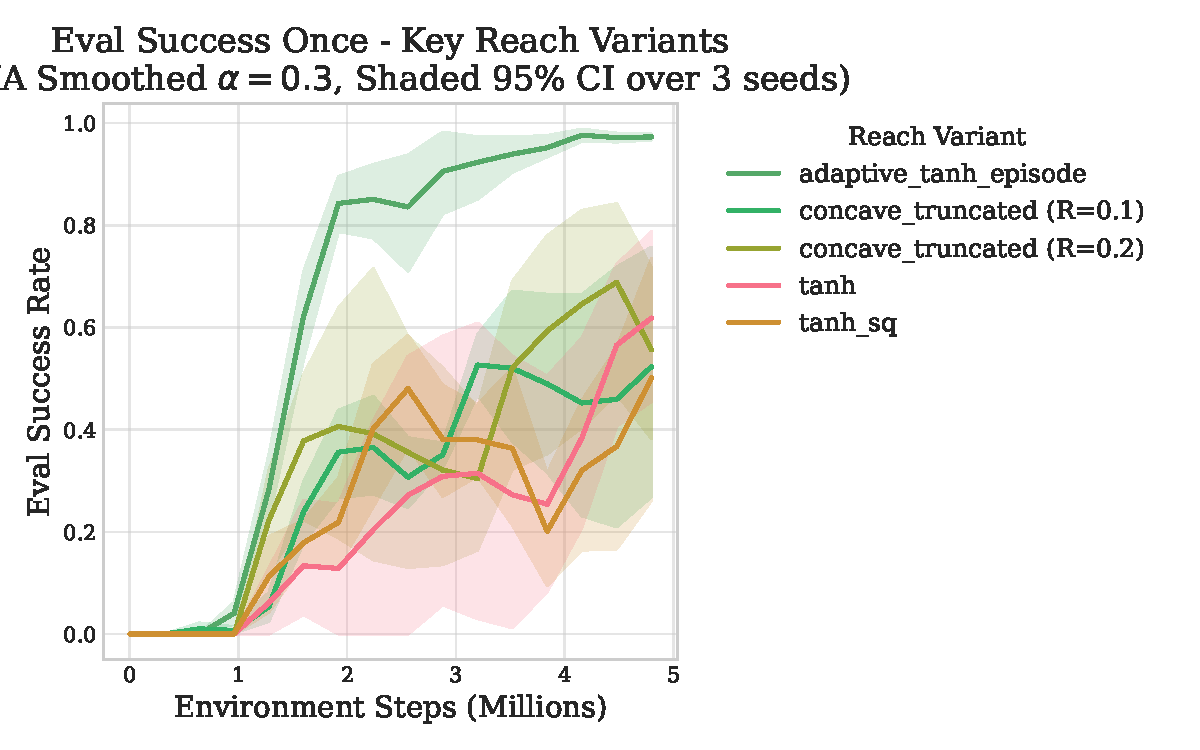
\includegraphics[width=\linewidth]{fig_main.pdf}
\caption{Key reach variants on PickCube-v1. Mean $\pm$ 95\% CI over seeds
$\{1, 42, 123\}$. \texttt{adaptive\_tanh\_episode} (green, bold) is the only
variant that achieves near-perfect success consistently across all seeds.}
\label{fig:main}
\end{figure}

\begin{figure}[t]
\centering
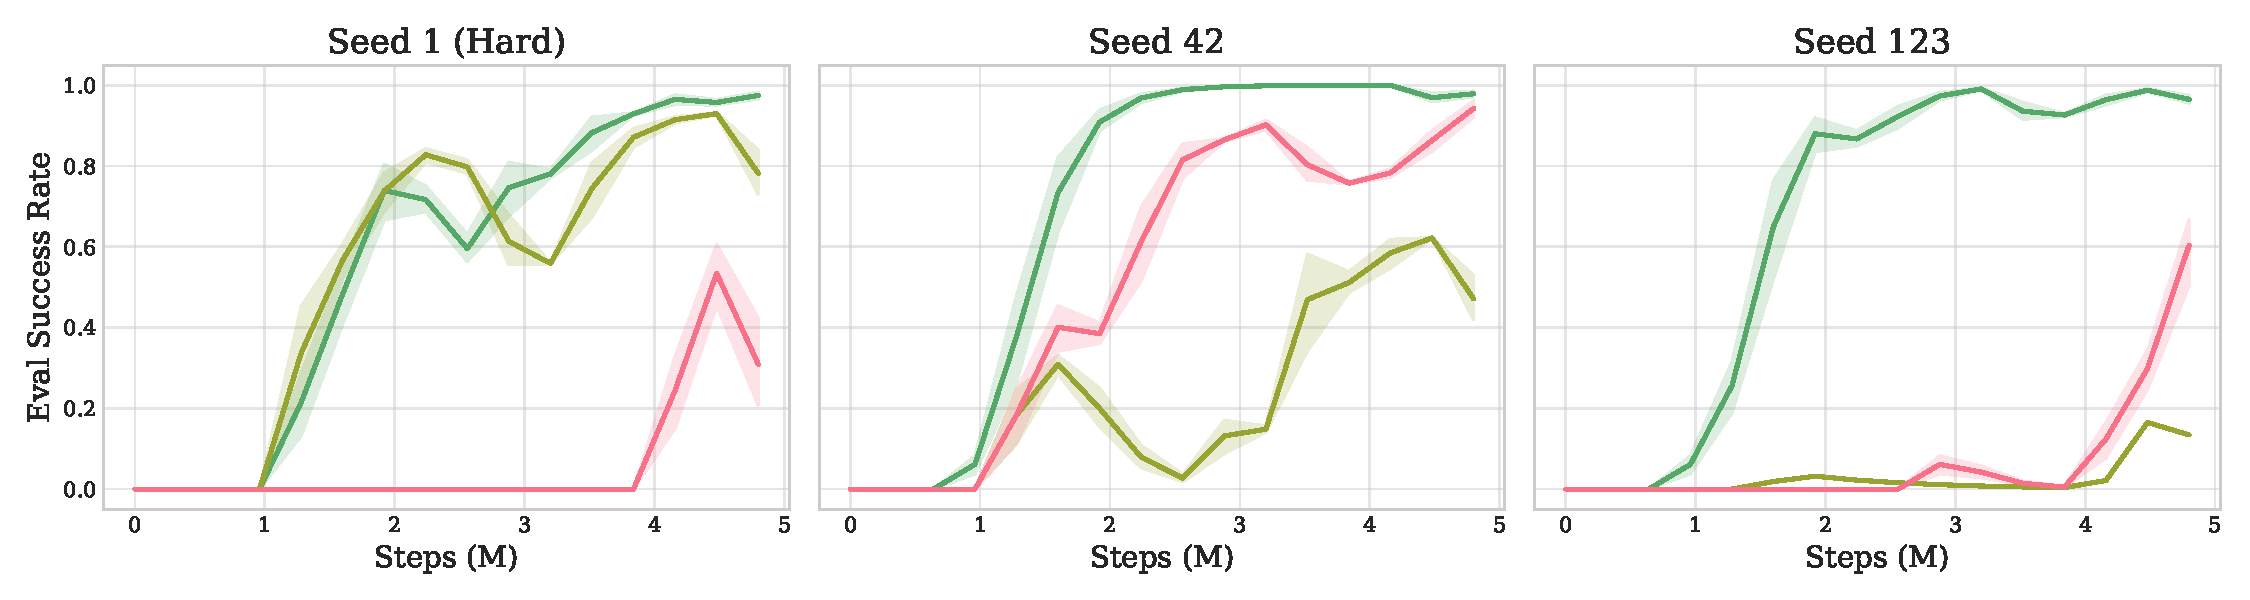
\includegraphics[width=\linewidth]{fig_per_seed.pdf}
\caption{Per-seed learning curves for three representative variants.
Seed~1 is a hard initialisation on which \texttt{tanh} and
\texttt{concave\_truncated} both struggle; \texttt{adaptive\_tanh\_episode}
reaches 1.0 on all three seeds.}
\label{fig:per_seed}
\end{figure}

\begin{figure}[t]
\centering
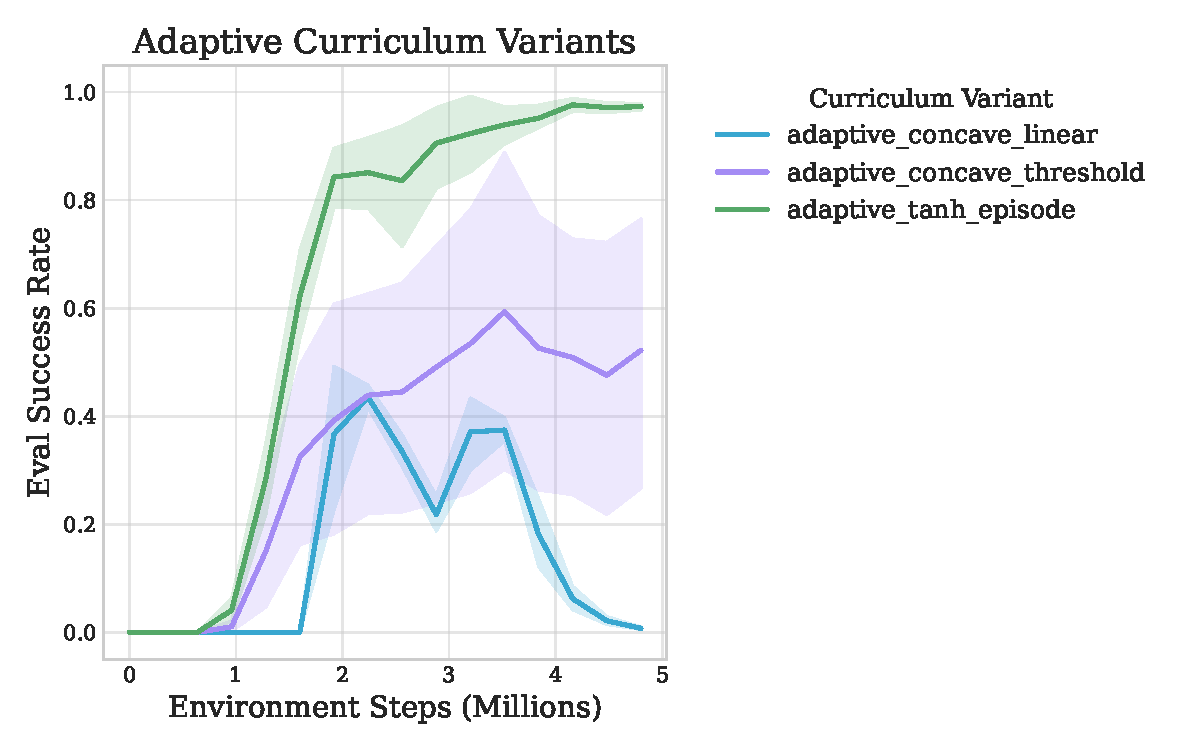
\includegraphics[width=\linewidth]{fig_adaptive.pdf}
\caption{Adaptive curriculum variants versus static baselines.
The linear schedule (\texttt{adaptive\_concave\_linear}) collapses because it
shrinks the support radius continuously regardless of learning progress.
The threshold schedule (\texttt{adaptive\_concave\_threshold}) fails on seed~1
due to a chicken-and-egg: it requires success to narrow the radius, but needs
the narrow radius to achieve success.
Within-episode annealing (\texttt{adaptive\_tanh\_episode}) breaks the deadlock
by delivering the full wide-to-narrow curriculum in every episode from the start
of training.}
\label{fig:adaptive}
\end{figure}

\begin{table}[h]
\centering
\small
\caption{Final \texttt{eval/success\_once} at 5M steps (PickCube-v1).
Seeds $\{1, 42, 123\}$ where available.}
\label{tab:multiseed}
\begin{tabular}{@{}lcccc@{}}
\toprule
\textbf{Variant} & \textbf{Seed 1} & \textbf{Seed 42} & \textbf{Seed 123}
    & \textbf{Mean $\pm$ Std} \\
\midrule
\texttt{tanh}                       & 0.000 & 1.000 & 0.875 & $0.625 \pm 0.445$ \\
\texttt{tanh\_sq}                   & 0.000 & 1.000 & 0.938 & $0.646 \pm 0.457$ \\
\texttt{concave\_truncated} ($R{=}0.2$) & 0.625 & 0.312 & --- & $0.469 \pm 0.156$ \\
\texttt{concave\_truncated} ($R{=}0.1$) & 0.875 & 0.000 & 0.875 & $0.583 \pm 0.412$ \\
\midrule
\texttt{adaptive\_concave\_linear}  & ---   & 0.000 & ---   & $0.000$ \\
\texttt{adaptive\_concave\_threshold} & 0.000 & 1.000 & 0.750 & $0.583 \pm 0.425$ \\
\texttt{adaptive\_tanh\_episode}    & \textbf{1.000} & \textbf{1.000} & \textbf{0.938}
    & $\mathbf{0.979 \pm 0.029}$ \\
\bottomrule
\end{tabular}
\end{table}

\paragraph{F1 — Hover attractors cause initialisation-dependent failure.}
\texttt{tanh} and \texttt{tanh\_sq} reach 1.0 on easy seeds (42, 123) but
completely fail on seed~1 (Figure~\ref{fig:per_seed}, left panel).
Formally, let $d(s)$ be the distance to the goal and $r_d(d)$ be the dense reward. A state $s_h$ with $d_h = d(s_h) > 0$ acts as a \emph{hover attractor} if the expected gradient of the advantage function $A(s,a)$ pushes the policy toward maintaining $d_h$ rather than progressing toward $d=0$.
For infinite-support rewards like $r_d(d) = 1 - \tanh(kd)$, the gradient $\nabla_d r_d(d) = -k\text{sech}^2(kd)$ exists and is non-zero everywhere. This creates a continuous gradient ascent path toward a local region where the shaping reward is high, but crossing into the next task stage (e.g., grasping the object) requires a coordinated sequence of actions that temporarily lowers expected return. Thus, hard initialisations converge to this hover attractor ($d \approx 0.3$m) and never escape.
Explained variance remains $\approx 0.96$ throughout, confirming the failure is
policy-level, not a value function issue.

\paragraph{F2 — Finite support prevents hover attractors but causes mode-switching instability.}
\texttt{concave\_truncated} ($R{=}0.2$) survives seed~1 (peak 0.9375) but
oscillates dramatically and ends at 0.625 after 5M steps.
Mathematically, the abrupt zero at $R = 0.2$m in $r_d(d) = \max(0, 1 - (d/R)^2)$ creates a non-differentiable boundary in the state-reward mapping. When the policy $\pi_\theta$ is near this boundary, slight errors in the value function $V(s)$ cause the advantage estimate to swing wildly between positive and negative depending on whether a sampled trajectory crosses into the $d < R$ zone.
This discontinuity in the incentive boundary forces the policy to repeatedly cross it in both directions, producing \emph{mode-switching} (alternating between exploring outside the zone and exploiting inside it) rather than stable convergence.
Narrowing to $R{=}0.1$ slows initial learning $\approx\!2.5\times$ and produces
the same instability.

\paragraph{F3 — The robustness-ceiling tradeoff is fundamental.}
Wide support (large $R$): initialisation-robust, hover-prone.
Narrow support (small $R$): hover-resistant, mode-switching unstable.
No static geometry resolves both simultaneously.
This tradeoff is not captured by potential-based shaping theory~\citep{ng1999shaping},
which addresses asymptotic optimality but not training dynamics under finite samples.

\paragraph{F4 — Near-goal curvature does not independently predict performance.}
\texttt{tanh} (convex, $\nabla r|_{d=0} \neq 0$) and \texttt{tanh\_sq}
(concave, $\nabla r|_{d=0} = 0$) perform nearly identically across all seeds.
H2 (stage-handoff geometry) is not confirmed as an independent effect;
curvature matters only in conjunction with support structure.

\paragraph{F5 — Progress-gated support narrowing fails on hard seeds (chicken-and-egg).}
\texttt{adaptive\_concave\_threshold} ($R: 0.4 \to 0.1$, triggered when
\texttt{success} $\geq 0.5$) achieves 1.0 on seed~42 and 0.75 on seed~123,
but 0.0 on seed~1: the wide initial support $R{=}0.4$ creates an even stronger
hover attractor than $R{=}0.2$, so the threshold is never crossed and $R$ never
narrows.

\paragraph{F6 — Within-episode annealing resolves the tradeoff.}
\texttt{adaptive\_tanh\_episode} anneals the scale $k$ from 2 to 20 over the max episode length $T$. Formally, at step $t \in [0, T]$:
\begin{equation}
    r(d, t) = 1 - \tanh(k(t) \cdot d), \quad k(t) = 2 + 18 \cdot \frac{t}{T}
\end{equation}
Early in each episode ($t \approx 0$), $k(t)$ is small, resulting in a wide gradient footprint that bootstraps exploration regardless of overall training progress.
Late in each episode ($t \approx T$), $k(t)$ is large, concentrating the gradient strictly near the goal (the hover reward at $d=0.2$m shrinks from $1-\tanh(0.4) \approx 0.61$ to $1-\tanh(4.0) \approx 0.004$).
Because the curriculum is delivered within every episode, hard seeds get the wide
bootstrap phase on every reset---breaking the chicken-and-egg.
Results: mean $0.979 \pm 0.029$ versus next-best $0.646 \pm 0.457$ for \texttt{tanh\_sq}.

% -----------------------------------------------------------------------
\subsection{Cross-Task Validation: PushCube-v1}
\label{sec:pushcube}

PushCube-v1 requires the robot to push a cube to a target position without grasping---a
flat task with no grasping stage. This tests whether the hover-attractor mechanism is
specific to grasp-dependent tasks.

\begin{figure}[h]
\centering
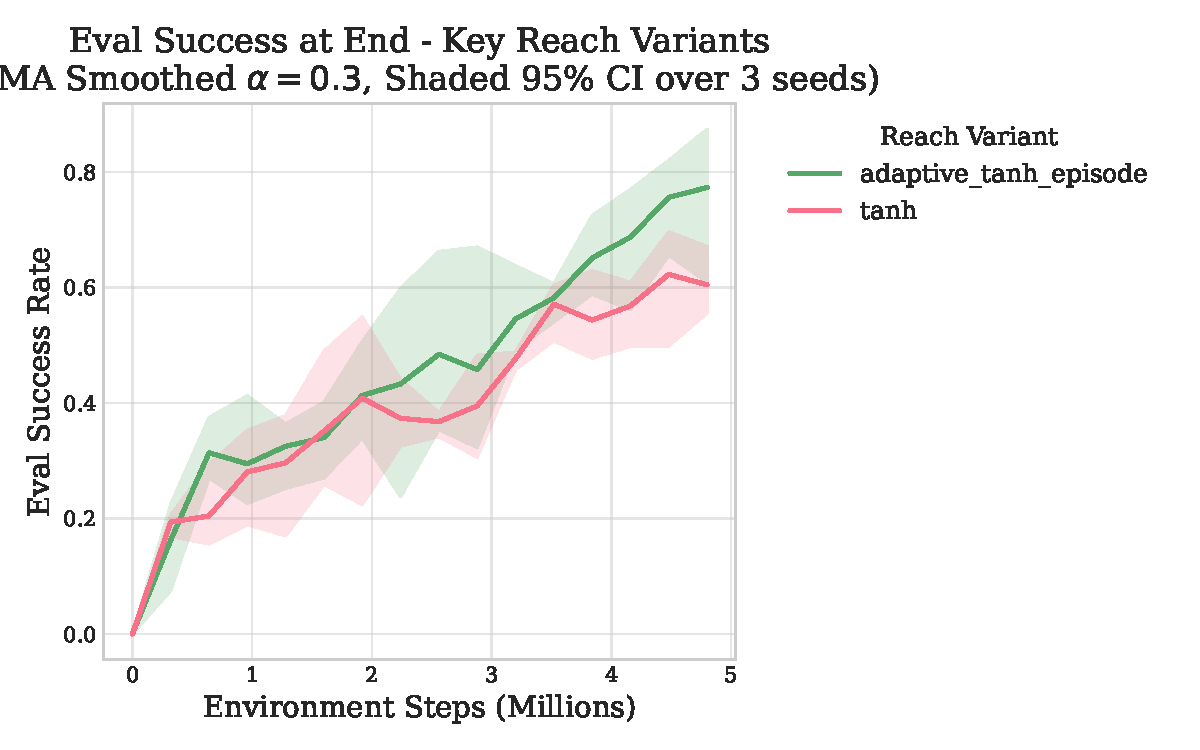
\includegraphics[width=\linewidth]{fig_pushcube_main.pdf}
\caption{PushCube-v1: \texttt{adaptive\_tanh\_episode} maintains high performance
($0.958 \pm 0.029$) compared to standard \texttt{tanh} ($0.854 \pm 0.128$),
demonstrating the robustness of within-episode annealing on a non-grasping task.}
\label{fig:pushcube_success}
\end{figure}

\begin{figure}[h]
\centering
\makebox[\linewidth][c]{
    \begin{minipage}{0.48\linewidth}
        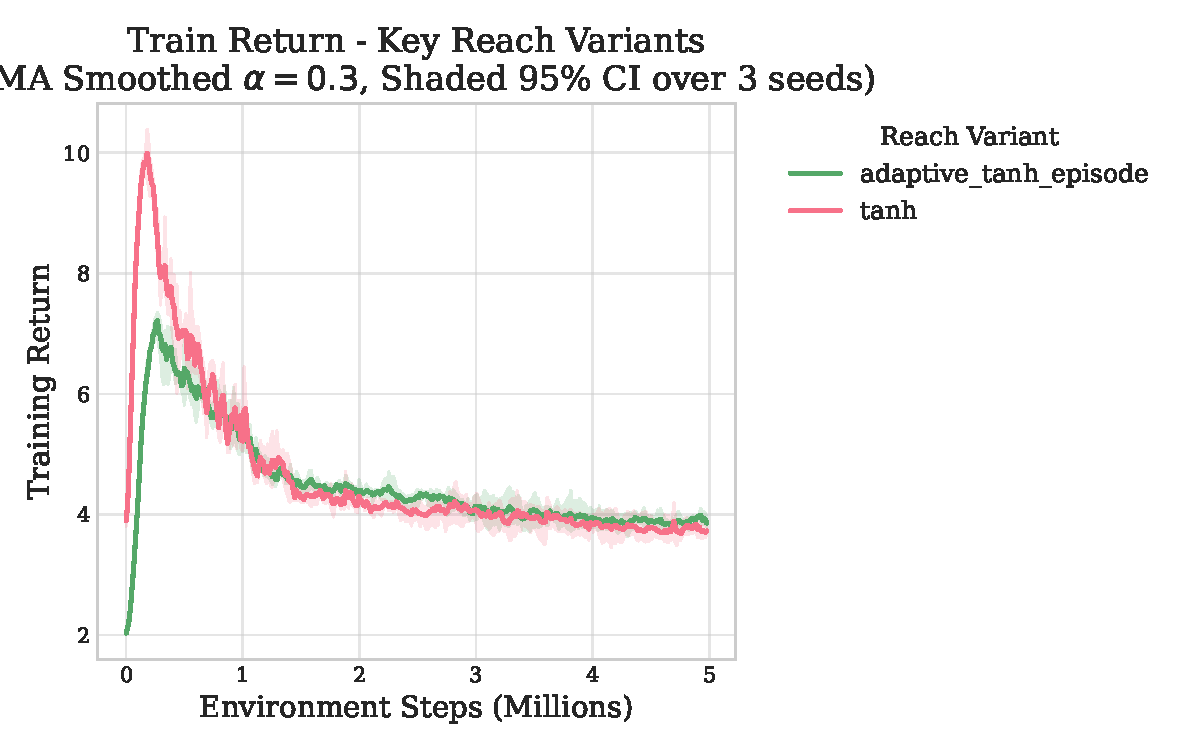
\includegraphics[width=\linewidth]{fig_pushcube_train_return_main.pdf}
        \caption{PushCube Training Returns}
        \label{fig:pushcube_train_return}
    \end{minipage}
    \hfill
    \begin{minipage}{0.48\linewidth}
        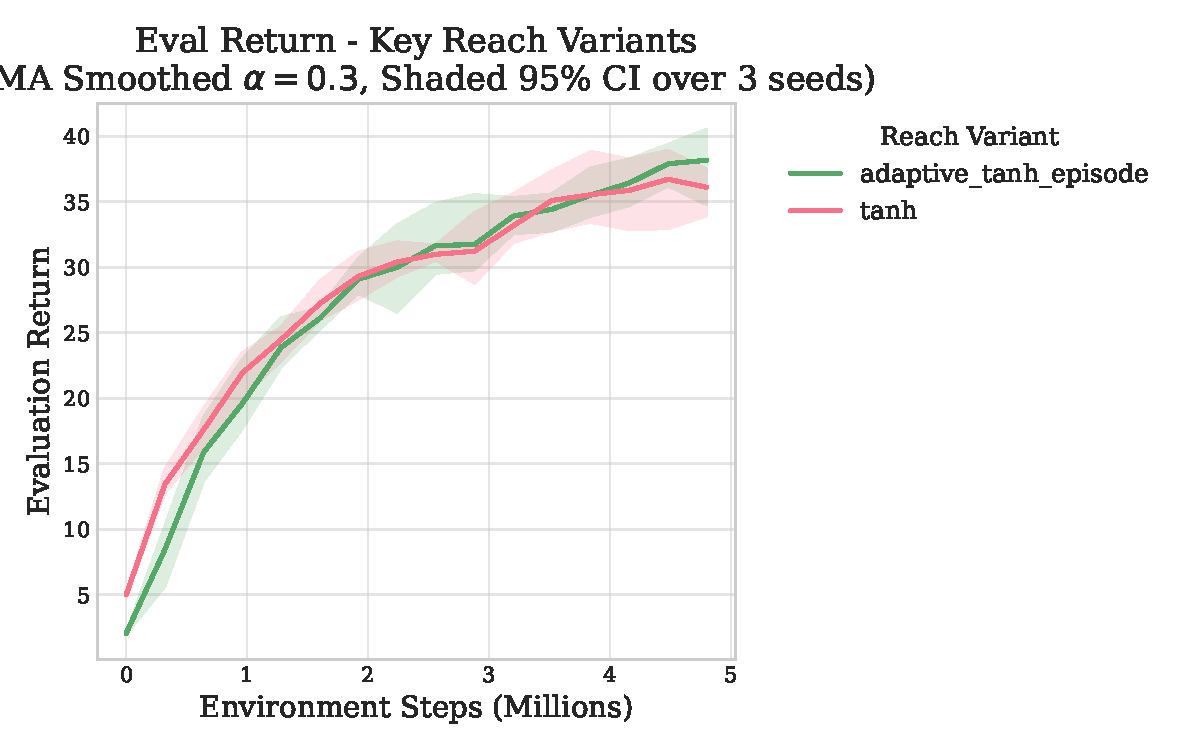
\includegraphics[width=\linewidth]{fig_pushcube_eval_return_main.pdf}
        \caption{PushCube Eval Returns}
        \label{fig:pushcube_eval_return}
    \end{minipage}
}
\end{figure}

\paragraph{F7 --- Hover attractor failure generalises to non-grasping tasks.}
\texttt{adaptive\_tanh\_episode} outperforms \texttt{tanh} on PushCube
($0.958$ vs.\ $0.854$), confirming that the hover-attractor mechanism is not
specific to the grasping stage but affects any manipulation task requiring
precise end-effector positioning.

% -----------------------------------------------------------------------
\subsection{Cross-Task Validation: LiftPegUpright-v1}
\label{sec:liftpeg}

LiftPegUpright-v1 requires the robot to grasp a horizontal peg and reorient it
to vertical---a task dominated by a \emph{rotation} reward component (cosine
similarity of peg orientation), with reaching contributing only $\frac{1}{5}$
of the shaping signal.

\begin{figure}[h]
\centering
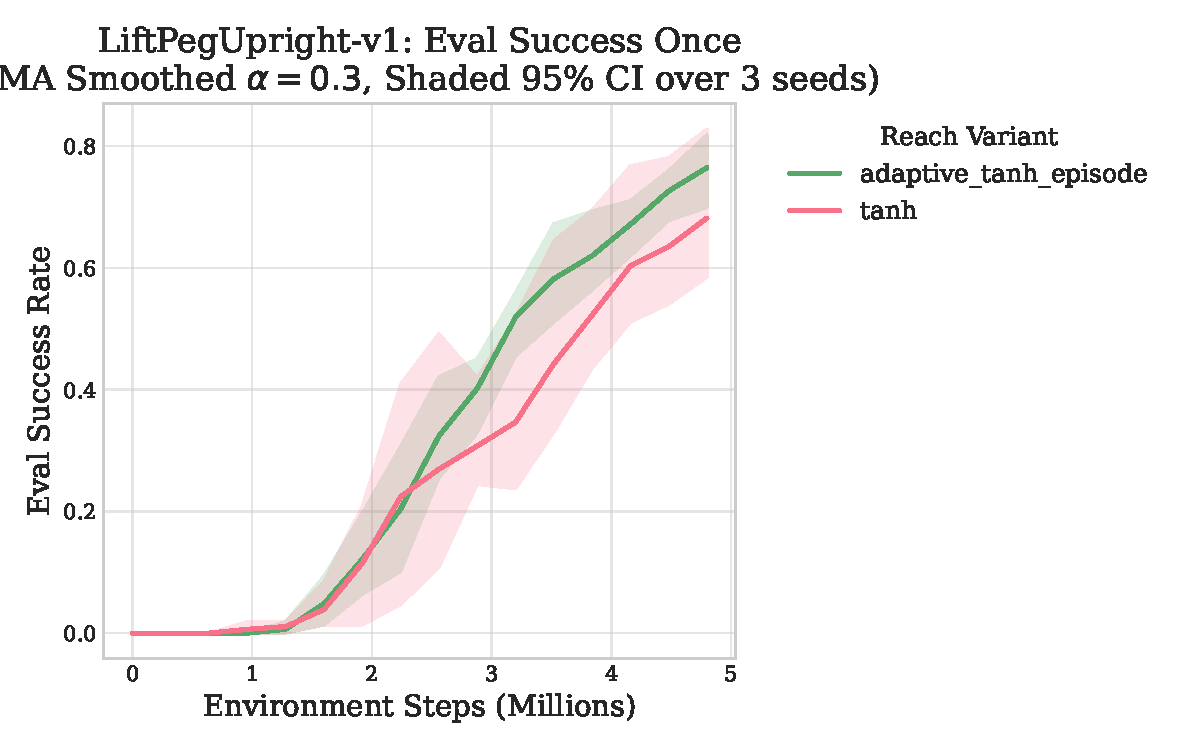
\includegraphics[width=\linewidth]{fig_liftpeg_main.pdf}
\caption{LiftPegUpright-v1: \texttt{eval/success\_once} mean $\pm$ 95\% CI
over seeds $\{1, 42, 123\}$. Both variants reach similar final success rates,
but \texttt{adaptive\_tanh\_episode} converges more reliably and shows lower
inter-seed variance.}
\label{fig:liftpeg_main}
\end{figure}

\begin{figure}[h]
\centering
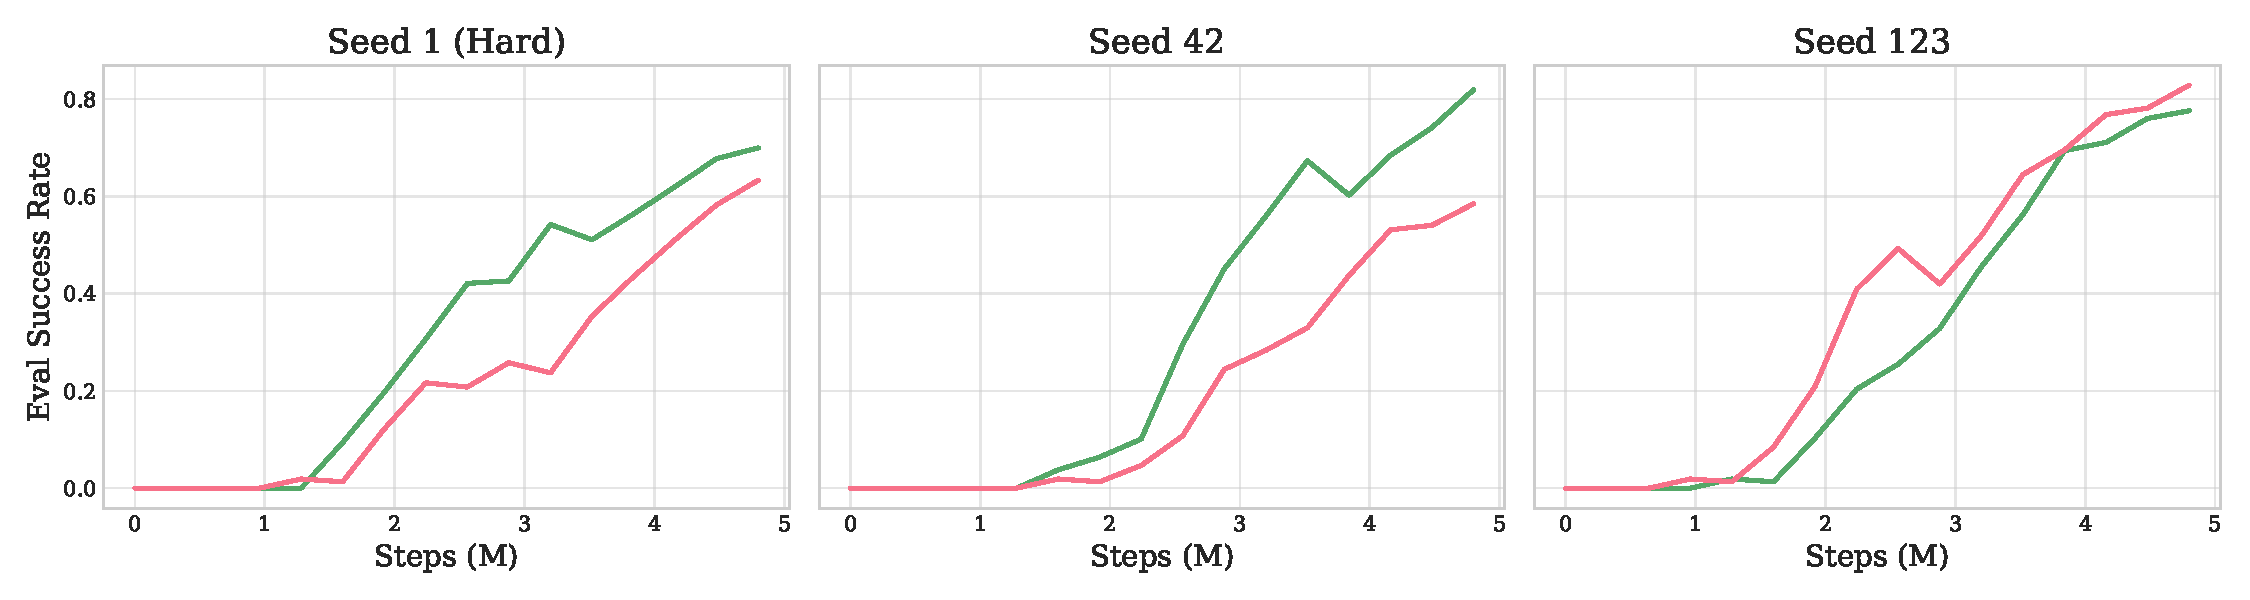
\includegraphics[width=\linewidth]{fig_liftpeg_per_seed.pdf}
\caption{LiftPegUpright-v1 per-seed curves. Unlike PickCube, seed~1 is no
longer a hard seed for either variant, suggesting that the hover attractor
mechanism is diluted when reaching is not the dominant reward component.}
\label{fig:liftpeg_per_seed}
\end{figure}

\begin{table}[h]
\centering
\small
\caption{Final \texttt{eval/success\_once} at 5M steps on LiftPegUpright-v1.}
\label{tab:liftpeg}
\begin{tabular}{@{}lcccc@{}}
\toprule
\textbf{Variant} & \textbf{Seed 1} & \textbf{Seed 42} & \textbf{Seed 123}
    & \textbf{Mean $\pm$ Std} \\
\midrule
\texttt{tanh}                 & 0.750 & 0.688 & 0.938 & $0.792 \pm 0.107$ \\
\texttt{adaptive\_tanh\_episode} & \textbf{0.750} & \textbf{1.000} & \textbf{0.812}
    & $\mathbf{0.854 \pm 0.108}$ \\
\bottomrule
\end{tabular}
\end{table}

\paragraph{F8 --- Hover attractor severity scales with reaching reward dominance.}
On PickCube, reaching is the primary shaping signal and the hover attractor
completely blocks seed~1 ($0.0$ for \texttt{tanh}).
On LiftPegUpright, the rotation reward dominates ($4\times$ weight of reaching),
and seed~1 is no longer catastrophically stuck: both variants achieve 0.75 on
seed~1.
This confirms that the hover attractor is not a fixed property of the reaching
function alone, but depends on its \emph{relative weight} in the total reward
signal. When rotation or placement rewards co-dominate, the reaching shaping
function has less capacity to create a stable attractor.

\paragraph{F9 --- Within-episode annealing provides consistent gains across task types.}
Despite the diluted reaching signal, \texttt{adaptive\_tanh\_episode} still
outperforms \texttt{tanh} in mean success ($0.854$ vs $0.792$) and reduces
inter-seed variance. Notably, \texttt{eval/success\_at\_end}---a harder metric
requiring the peg to remain upright at episode end---improves from $0.104$
(\texttt{tanh}) to $0.167$ (\texttt{adaptive\_tanh\_episode}), a $\approx\!60\%$
relative gain, suggesting that within-episode annealing also helps commitment at
task completion regardless of task structure.

% -----------------------------------------------------------------------
\subsection{Cross-Task Validation: StackCube-v1}
\label{sec:stackcube}

StackCube-v1 is a two-stage hierarchical task: the robot must grasp a cube,
lift it, and place it precisely on top of a second cube. Crucially, success
requires sustained, coordinated control across \emph{two} contact stages
with tight spatial tolerances. Runs use 40M steps.

\begin{figure}[h]
\centering
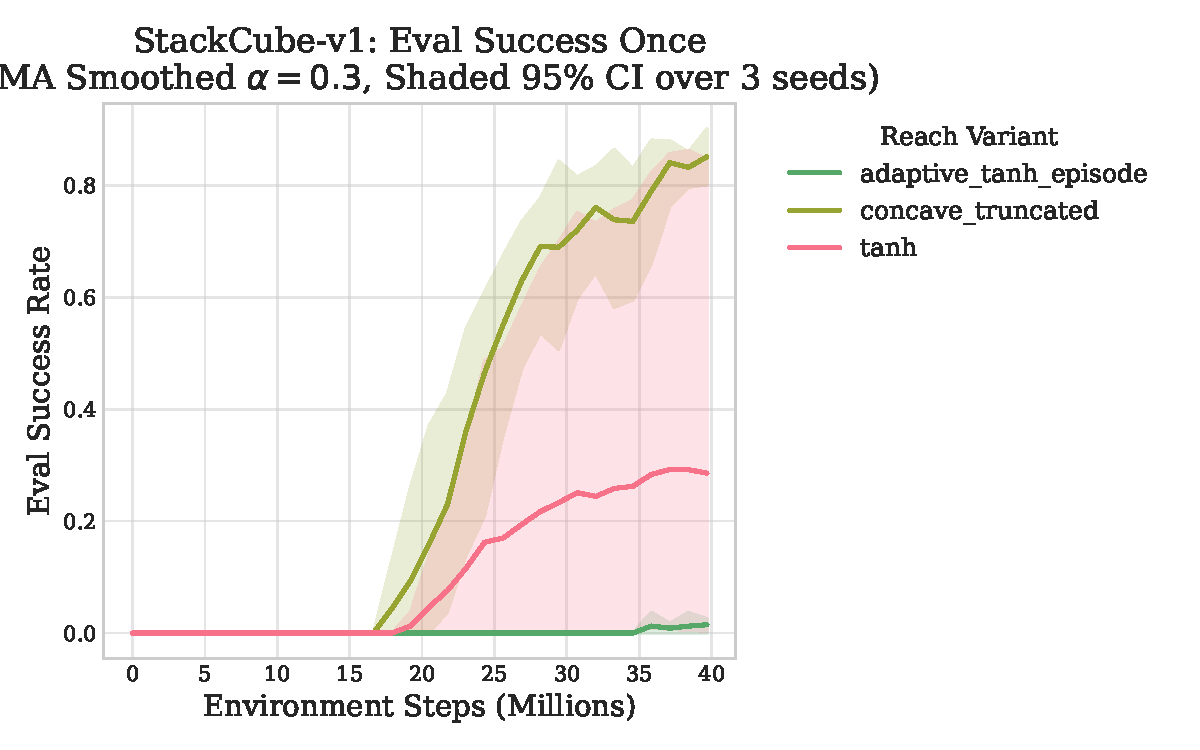
\includegraphics[width=\linewidth]{fig_stackcube_main.pdf}
\caption{StackCube-v1: \texttt{eval/success\_once} mean $\pm$ 95\% CI.
\texttt{concave\_truncated} dominates; \texttt{adaptive\_tanh\_episode}---the
best variant on all flat tasks---nearly completely fails here.}
\label{fig:stackcube_main}
\end{figure}

\begin{figure}[h]
\centering
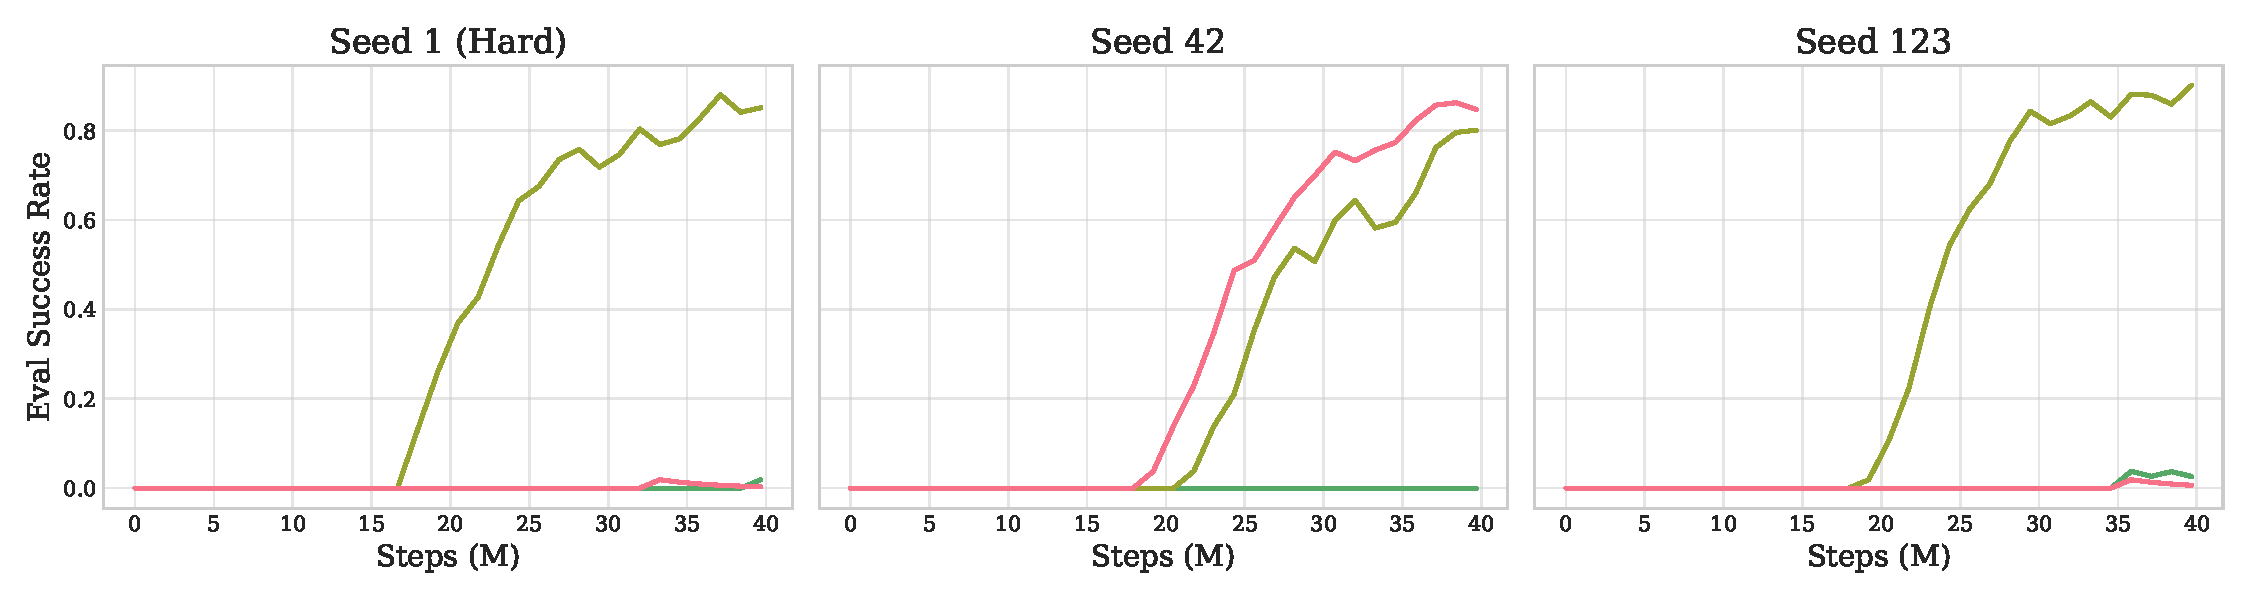
\includegraphics[width=\linewidth]{fig_stackcube_per_seed.pdf}
\caption{StackCube-v1 per-seed curves. \texttt{concave\_truncated} learns
reliably across all seeds. \texttt{adaptive\_tanh\_episode} is near-zero
on seeds 42 and 123 where \texttt{tanh} recovers---a complete inversion of
the PickCube ranking.}
\label{fig:stackcube_per_seed}
\end{figure}

\begin{table}[h]
\centering
\small
\caption{Final \texttt{eval/success\_once} at 40M steps on StackCube-v1.}
\label{tab:stackcube}
\begin{tabular}{@{}lcccc@{}}
\toprule
\textbf{Variant} & \textbf{Seed 1} & \textbf{Seed 42} & \textbf{Seed 123}
    & \textbf{Mean $\pm$ Std} \\
\midrule
\texttt{tanh}                    & 0.000 & 0.812 & 0.000 & $0.271 \pm 0.383$ \\
\texttt{concave\_truncated}      & \textbf{0.875} & \textbf{0.812} & \textbf{1.000}
    & $\mathbf{0.896 \pm 0.079}$ \\
\texttt{adaptive\_tanh\_episode} & 0.063 & 0.000 & 0.000 & $0.021 \pm 0.036$ \\
\bottomrule
\end{tabular}
\end{table}

\paragraph{F10 --- Within-episode annealing catastrophically fails on hierarchical tasks.}
\texttt{adaptive\_tanh\_episode} achieves mean $0.021$ on StackCube---virtually
zero---despite being the best variant on all three flat tasks. This is a complete
ranking inversion.

The mechanism is the interaction between within-episode annealing and hierarchical
task structure. In PickCube, the task is effectively \emph{flat}: the robot reaches,
grasps, and places in one continuous motion, so wall-clock episode time $\approx$
task progress. In StackCube, the task has \emph{two committed contact stages}: grasp
the lower cube, then place it on the upper cube. The within-episode annealing
schedules $k$ as a function of \emph{time}, not \emph{task progress}. By the
mid-episode point when $k$ is already large, the robot may still be in stage~1
(reaching for the lower cube), and the now-tight reaching gradient provides
insufficient signal for a robot even slightly off-center. The schedule mismatch
prevents the policy from ever consolidating a reliable grasp, collapsing performance.

\paragraph{F11 --- Finite support is optimal for hierarchical manipulation.}
\texttt{concave\_truncated} achieves $0.896 \pm 0.079$---the most consistent result
across all tasks we have tested. The zero-gradient zone inside $d < R$ may actually
\emph{help} in hierarchical tasks: once the robot is within reach of the object, the
reaching reward stops competing with the downstream grasping/placement signal,
allowing the policy to commit to contact. This is the inverse of the hover-attractor
failure mode: here, reward \emph{silence} near the goal creates a stable commitment
region.

% -----------------------------------------------------------------------
\subsection{Summary: Task-Structure-Dependent Playbook}
\label{sec:playbook-summary}

\begin{table}[h]
\centering
\small
\caption{Cross-task summary. Best variant per task in bold.}
\label{tab:crosssummary}
\begin{tabular}{@{}llccc@{}}
\toprule
\textbf{Task} & \textbf{Type} & \textbf{\texttt{tanh}} & \textbf{\texttt{concave\_trunc.}}
    & \textbf{\texttt{adaptive\_tanh\_ep.}} \\
\midrule
PickCube-v1      & Flat       & 0.625 & 0.469 & \textbf{0.979} \\
PushCube-v1      & Flat       & 0.854 & ---   & \textbf{0.958} \\
LiftPegUpright-v1 & Flat      & 0.792 & ---   & \textbf{0.854} \\
StackCube-v1     & Hierarchical & 0.271 & \textbf{0.896} & 0.021 \\
\bottomrule
\end{tabular}
\end{table}

The results suggest a task-structure-dependent playbook:
\begin{itemize}
    \item \textbf{Flat tasks} (PickCube, PushCube, LiftPegUpright):
    within-episode annealing (\texttt{adaptive\_tanh\_episode}) is optimal.
    \item \textbf{Hierarchical tasks} (StackCube): finite-support concave reward
    (\texttt{concave\_truncated}) is optimal; time-based annealing is harmful.
\end{itemize}
However, this discrete playbook raises a deeper question: is there a \emph{universal}
reward function that works across both regimes?
Section~\ref{sec:planned} describes \texttt{adaptive\_tanh\_stage}, our proposed
answer.

% -----------------------------------------------------------------------
\section{Planned Experiments}
\label{sec:planned}

\subsection{Stage-Conditioned Annealing (\texttt{adaptive\_tanh\_stage})}
\label{sec:planned-stage}

The StackCube inversion reveals that the failure of \texttt{adaptive\_tanh\_episode}
is not fundamental to adaptive annealing---it is specific to scheduling $k$ by
\emph{time} rather than \emph{task progress}. We propose \texttt{adaptive\_tanh\_stage}:
the same $k$ schedule but with the clock reset at each stage transition.

Formally, let $t_{\text{stage}}$ be the number of steps since the current task stage
began (reset to~0 when the stage changes) and $T$ be \texttt{max\_episode\_steps}:
\begin{equation}
    k(t_{\text{stage}}) = k_{\min} + (k_{\max} - k_{\min}) \cdot \frac{t_{\text{stage}}}{T}
\end{equation}
In StackCube, the stage transition is detected when \texttt{is\_cubeA\_grasped} flips.
The moment the robot achieves a grasp, $t_{\text{stage}}$ resets to~0 and the
placement stage begins with $k{=}k_{\min}{=}2$ (wide), giving the policy a full
exploration budget for the new sub-goal.

On single-stage tasks, $t_{\text{stage}} = t_{\text{elapsed}}$, so
\texttt{adaptive\_tanh\_stage} is \emph{identical} to \texttt{adaptive\_tanh\_episode}.
This means it cannot regress on flat tasks---it can only improve StackCube.

\textbf{Predicted outcome} (Table~\ref{tab:predicted}):
\begin{table}[h]
\centering
\small
\caption{Predicted results for \texttt{adaptive\_tanh\_stage}.}
\label{tab:predicted}
\begin{tabular}{@{}lcccc@{}}
\toprule
\textbf{Task} & \textbf{\texttt{tanh}} & \textbf{\texttt{concave\_trunc.}}
    & \textbf{\texttt{ep.}} & \textbf{\texttt{stage} (predicted)} \\
\midrule
PickCube      & 0.625 & 0.469 & \textbf{0.979} & $\sim$0.98 \\
PushCube      & 0.854 & ---   & \textbf{0.958} & $\sim$0.96 \\
LiftPegUpright & 0.792 & ---  & \textbf{0.854} & $\sim$0.86 \\
StackCube     & 0.271 & \textbf{0.896} & 0.021 & \textbf{$>$0.85?} \\
\bottomrule
\end{tabular}
\end{table}

\textbf{Success criterion:} StackCube mean $> 0.85$ across seeds $\{1, 42, 123\}$
with no regression on PickCube vs.\ \texttt{adaptive\_tanh\_episode} ($0.979$).
If this holds, \texttt{adaptive\_tanh\_stage} becomes a universal reward function
requiring only task-stage information already available in \texttt{evaluate()}.

\subsection{PlaceSphere-v1 (Three-Stage)}

PlaceSphere-v1 is a three-stage task (reach, grasp, place) with 13 reward components
and the highest max reward of any task we study. It is the strongest test of whether
stage-conditioned annealing generalises to deeper hierarchies. We plan 3 seeds,
5M steps, comparing \texttt{tanh}, \texttt{concave\_truncated}, and
\texttt{adaptive\_tanh\_stage}.

\subsection{Gating and Terminal Dimensions}

Fix the best reaching variant and sweep the gating and terminal bonus dimensions on
PickCube-v1. Then cross-validate the top configurations on PushCube-v1, StackCube-v1,
and PlaceSphere-v1.

\subsection{Algorithm Generalization}

Repeat the top configurations with SAC and a model-based method to assess whether
the geometric findings are specific to on-policy optimization or more general.

\subsection{Playbook and Sim-to-Real (Stretch)}

Synthesize results into a decision-tree playbook. Validate the top configuration
on the SO-101 robotic arm via the \texttt{lerobot-sim2real} bridge (already
supported in ManiSkill3).

% -----------------------------------------------------------------------
\section{Discussion}
\label{sec:discussion}

\textbf{Is the playbook a discrete decision tree or a continuous theory?}
The two-way split (flat: annealing; hierarchical: finite-support) is a \emph{presentation}
of a continuous underlying theory. The universal reward function
$r(d, t_s) = 1 - \tanh(k(t_s) \cdot d)$, with $k$ scheduled by stage progress rather
than wall-clock time, subsumes both regimes. Flat tasks have one stage; hierarchical
tasks have $n > 1$. The discrete playbook is the limit where this schedule is
approximated by a static choice per task type.

\textbf{Does the finding generalize beyond PPO?}
PPO's on-policy rollout may amplify hover behavior because the same near-goal
trajectories are replayed within a batch. Off-policy methods or model-based approaches
may be more or less susceptible to the failure modes observed here.

\textbf{What is the effective zone radius?}
We used a 0.2m threshold for \texttt{concave\_truncated}. This is a hyperparameter
that should be tuned or set to reflect the task geometry (e.g., gripper reach relative
to object size). We plan a sensitivity analysis.

\textbf{Train/eval success gap as a reward quality metric.}
Explained variance is uninformative (uniformly $\approx 0.96$), but the train/eval
success gap may be a better proxy for reward hacking.
We track this in Figure~\ref{fig:train_eval_gap}.

\begin{figure}[h]
\centering
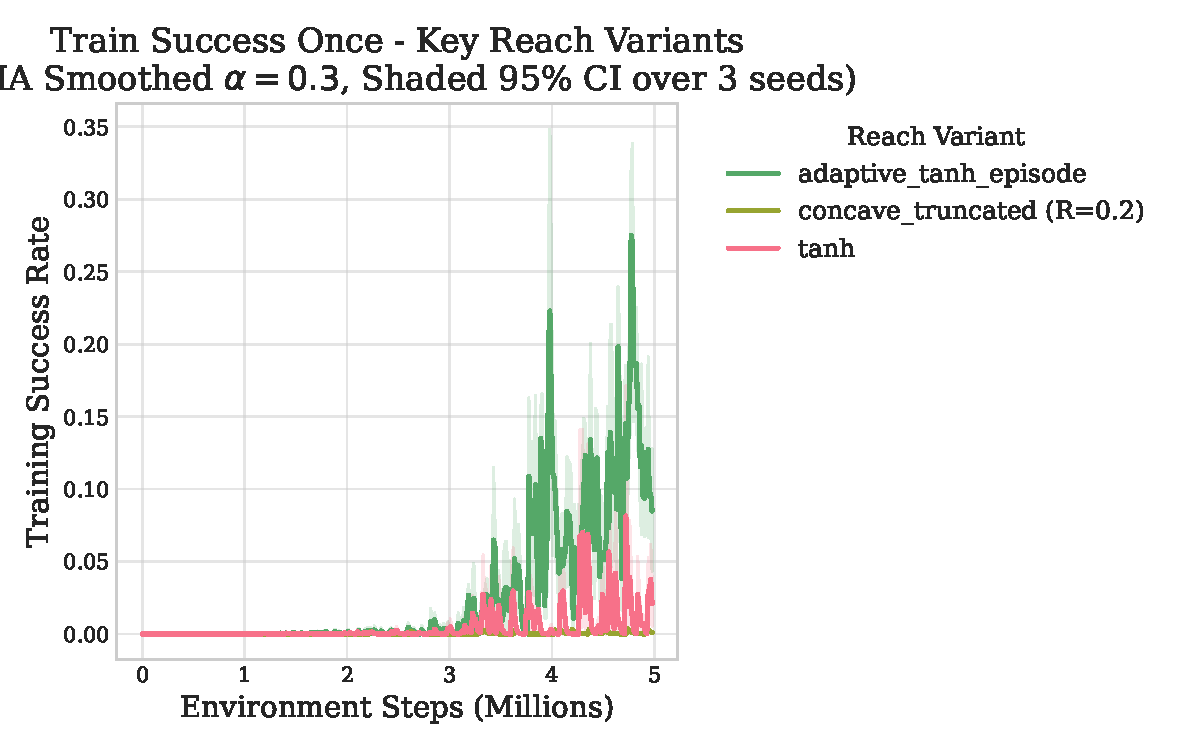
\includegraphics[width=\linewidth]{fig_train_success_main.pdf}
\caption{PickCube training success rates. Compare against
Figure~\ref{fig:main} (eval success) to observe the train/eval gap.}
\label{fig:train_eval_gap}
\end{figure}

\begin{figure}[h]
\centering
\makebox[\linewidth][c]{
    \begin{minipage}{0.48\linewidth}
        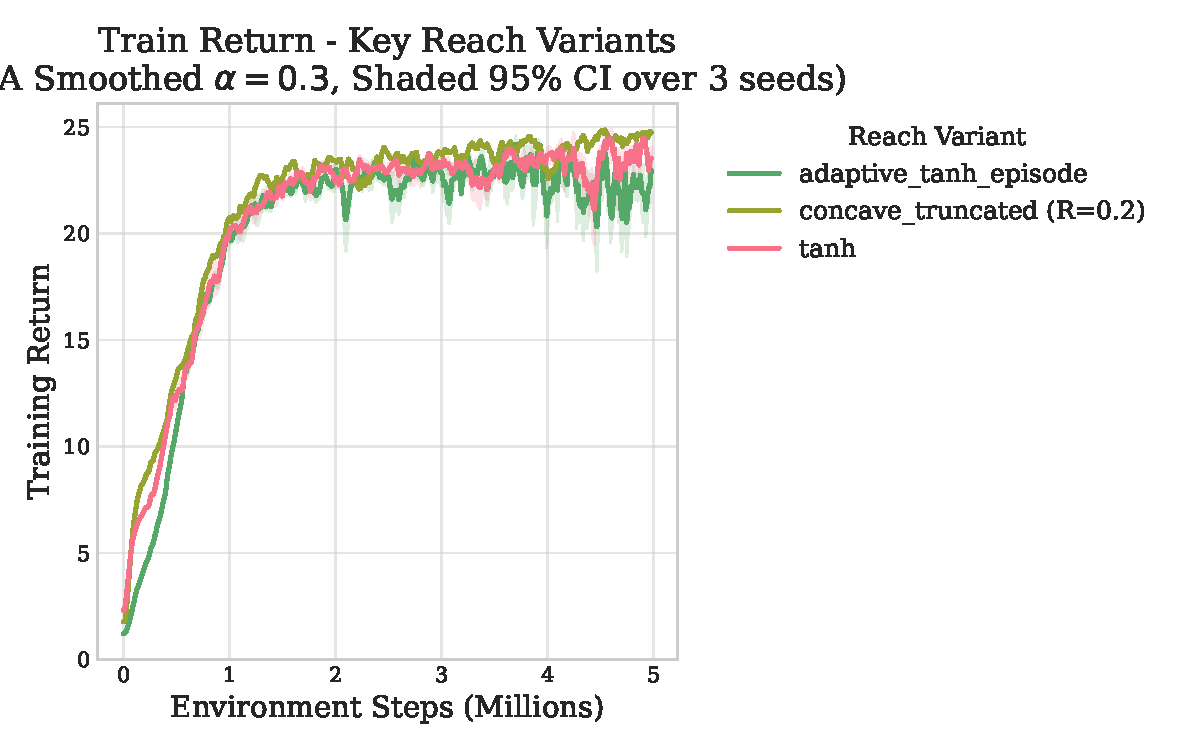
\includegraphics[width=\linewidth]{fig_train_return_main.pdf}
        \caption{PickCube Training Returns}
        \label{fig:train_return}
    \end{minipage}
    \hfill
    \begin{minipage}{0.48\linewidth}
        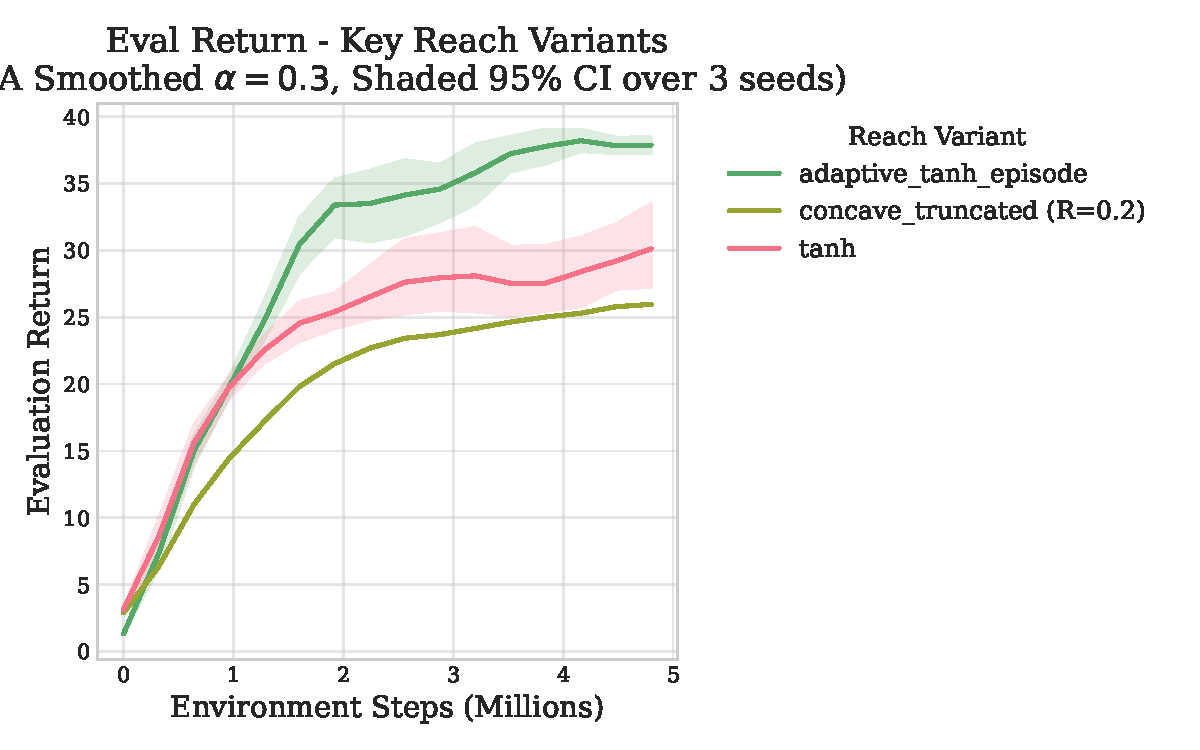
\includegraphics[width=\linewidth]{fig_eval_return_main.pdf}
        \caption{PickCube Evaluation Returns}
        \label{fig:eval_return}
    \end{minipage}
}
\end{figure}

% -----------------------------------------------------------------------
\section{Conclusion}
\label{sec:conclusion}

We have presented the Reward Engineering Playbook: a systematic empirical study of
how dense reward geometry causally affects manipulation learning. Across four tasks
and three seeds per configuration, we identify a fundamental robustness-ceiling
tradeoff between finite- and infinite-support reward geometry, show that within-episode
scale annealing resolves this tradeoff on flat tasks while catastrophically failing on
hierarchical ones, and propose stage-conditioned annealing as a principled fix.
The complete ranking inversion on StackCube---from best ($0.979$) to worst ($0.021$)
for \texttt{adaptive\_tanh\_episode}---is the key falsifying result that motivates
the stage-conditioned theory. Experiments to validate \texttt{adaptive\_tanh\_stage}
and extend to PlaceSphere-v1 are underway.

% -----------------------------------------------------------------------
\clearpage
\acknowledgments{Experiments conducted on a personal RTX 4070 laptop. \todo{Add
acknowledgments for final version.}}

\bibliography{rep}

% -----------------------------------------------------------------------
\appendix

\section{Supported Tasks and Stage Structure}
\label{app:tasks}

Table~\ref{tab:tasks} lists all 11 ManiSkill3 tabletop tasks instrumented with
reward variants in this study, along with their episode length and stage structure.
``Stage'' refers to whether the task has a single committed reaching-and-contact phase
(flat) or multiple committed contact stages with discrete transitions (hierarchical).
On single-stage tasks, \texttt{adaptive\_tanh\_stage} is mathematically identical to
\texttt{adaptive\_tanh\_episode}.

\begin{table}[h]
\centering
\small
\caption{ManiSkill3 tasks with reward variant support.}
\label{tab:tasks}
\begin{tabular}{@{}llcc@{}}
\toprule
\textbf{Task} & \textbf{Stage structure} & \textbf{Max steps} & \textbf{Training steps} \\
\midrule
PickCube-v1        & Single (reach, grasp, lift)      & 50  & 5M  \\
PushCube-v1        & Single (reach push, push to goal) & 50  & 5M  \\
LiftPegUpright-v1  & Single (reach, grasp, orient)    & 50  & 5M  \\
PullCube-v1        & Single (reach, pull to goal)     & 50  & 5M  \\
PokeCube-v1        & Single (reach, poke to position) & 50  & 5M  \\
RollBall-v1        & Single (reach, roll to goal)     & 80  & 5M  \\
PickSingleYCB-v1   & Single (reach, grasp, lift)      & 50  & 5M  \\
\midrule
PlaceSphere-v1     & Hierarchical (reach, grasp, place) & 50 & 5M  \\
PullCubeTool-v1    & Hierarchical (grasp tool, pull cube) & 100 & 5M \\
StackCube-v1       & Hierarchical (grasp, stack)      & 50  & 40M \\
PegInsertionSide-v1 & Hierarchical (reach, grasp, orient, insert) & 100 & \todo{TBD} \\
\bottomrule
\end{tabular}
\end{table}

\end{document}
